% Created 2021-03-03 Wed 21:13
% Intended LaTeX compiler: pdflatex
\documentclass[presentation]{beamer}
\usepackage[utf8]{inputenc}
\usepackage[T1]{fontenc}
\usepackage{graphicx}
\usepackage{grffile}
\usepackage{longtable}
\usepackage{wrapfig}
\usepackage{rotating}
\usepackage[normalem]{ulem}
\usepackage{amsmath}
\usepackage{textcomp}
\usepackage{amssymb}
\usepackage{capt-of}
\usepackage{hyperref}
\usepackage{minted}
\usepackage[utf8]{inputenc}
\usepackage{color}
\usetheme[height=7mm]{Rochester}
\setbeamertemplate{footline}[frame number]
\usecolortheme[accent=red, light]{solarized}
\setbeamercolor{frametitle}{bg=solarizedRebase02,fg=solarizedAccent}
\setbeamercolor{author in head/foot}{bg=solarizedRebase02,fg=solarizedRebase01}
\setbeamercolor{title in head/foot}{bg=solarizedRebase02,fg=solarizedRebase01}
\setbeamercolor{block title}{bg=solarizedRebase0,fg=solarizedRebase02}
\setbeamercolor{block body}{bg=solarizedRebase02,fg=solarizedRebase0}
\setbeamercolor{item}{bg=solarizedRebase02,fg=solarizedAccent}
\beamertemplatenavigationsymbolsempty
\usemintedstyle{manni}
\AtBeginSection[]{
\begin{frame}
\vfill
\centering
\begin{beamercolorbox}[sep=8pt,center,shadow=true,rounded=true]{title}
\Huge\insertsectionhead\par%
\end{beamercolorbox}
\vfill
\end{frame}
}
\usetheme{default}
\author{Sebastian Stabinger, Thomas Hausberger}
\date{SS2021}
\title{Dynamische Speicherverwaltung}
\hypersetup{
 pdfauthor={Sebastian Stabinger, Thomas Hausberger},
 pdftitle={Dynamische Speicherverwaltung},
 pdfkeywords={},
 pdfsubject={},
 pdfcreator={Emacs 27.1 (Org mode 9.4.4)},
 pdflang={Ger}}
\begin{document}

\maketitle
\section{Stack vs. Heap}
\label{sec:orgd72c2d1}
\begin{frame}[label={sec:org84ec29e}]{Stack vs. Heap}
\begin{block}{Stack}
\begin{itemize}
\item Enthält lokale Variablen, übergebene Parameter, intern benötigte
Informationen (z.B. Rücksprungadresse beim Aufruf von Funktionen, \ldots{})
\item Wird vom Compiler/System \alert{automatisch verwaltet}
\item In der Größe beschränkt
\end{itemize}
\end{block}
\begin{block}{Heap}
\begin{itemize}
\item Muss vom Programmierer manuell verwaltet werden
\item Es kann so viel Speicher verwendet werden wie das System erlaubt
(RAM, Swap, \ldots{})
\end{itemize}
\end{block}
\end{frame}
\begin{frame}[label={sec:org01f9449}]{Stack (Stapel) --- Datenstruktur}
\begin{columns}
\begin{column}{0.4\columnwidth}
\begin{itemize}
\item Häufig verwendete Datenstruktur
\item Wir können Elemente oben auf einen Stapel legen (push)
\item Wir können das oberste Element des Stapels entfernen (pop)
\end{itemize}
\end{column}
\begin{column}{0.6\columnwidth}
\begin{center}\begin{center}
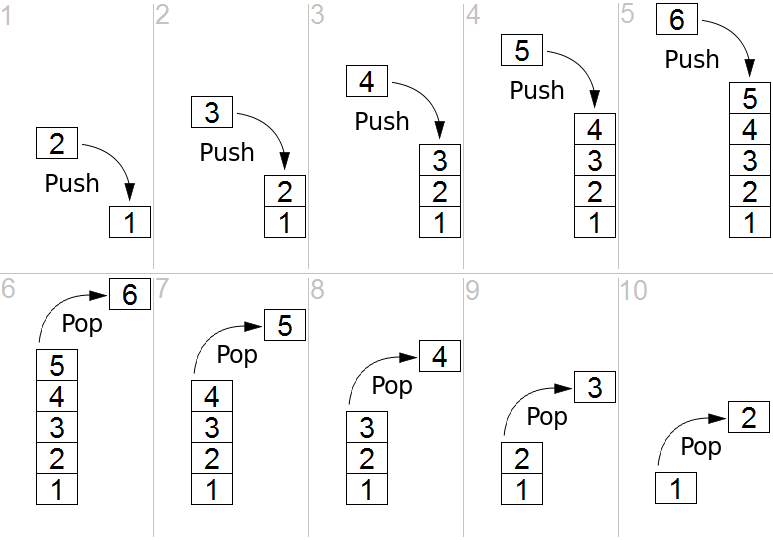
\includegraphics[width=.9\linewidth]{images/Lifo_stack.png}
\end{center}\end{center}
\end{column}
\end{columns}
\end{frame}
\begin{frame}[label={sec:org8231ffb},fragile]{Stack (Stapel) --- Verwaltung von Speicher von Funktionen}
 \begin{columns}
\begin{column}{0.5\columnwidth}
\begin{itemize}
\item Sämtlicher Speicher der für eine Funktion benötigt wird bezeichnet
man als \alert{Stackframe}
\item Diese Stackframes werden auf einem Stack verwaltet
\item Wird eine \alert{Funktion aufgerufen}, kommt ein \alert{neuer Stackframe auf den
Stapel}
\item Wenn eine \alert{Funktion fertig} ist ({\color{solarizedYellow}\texttt{return}}), wird der oberste
Stackframe vom Stapel \alert{entfernt}
\end{itemize}
\end{column}
\begin{column}{0.5\columnwidth}
\begin{center}\begin{center}
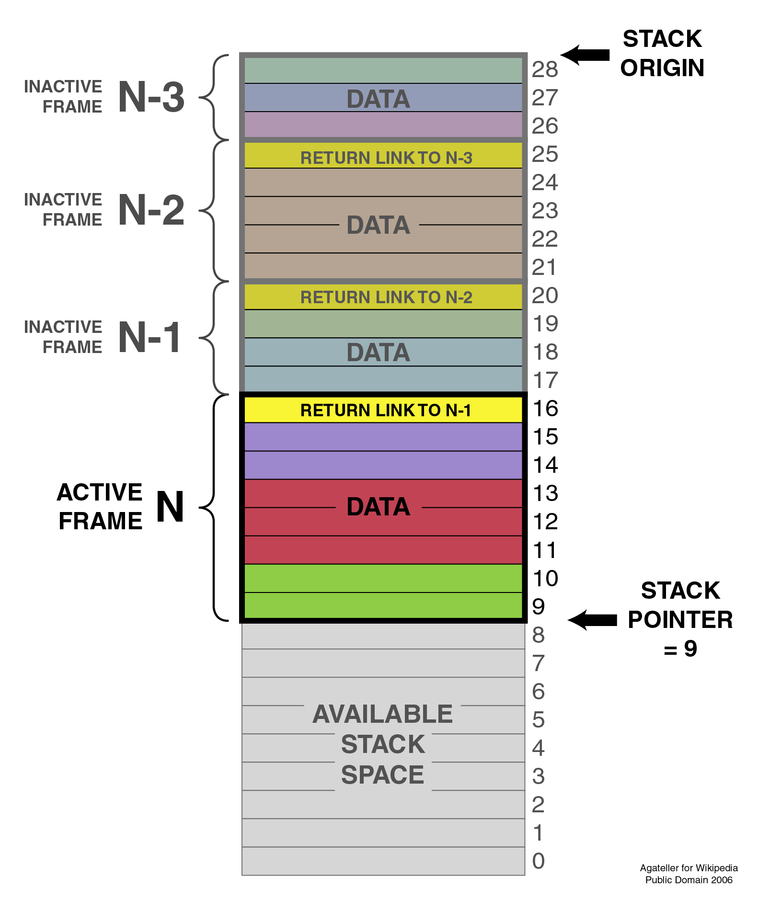
\includegraphics[width=.9\linewidth]{images/ProgramCallStack2_en.png}
\end{center}\end{center}
\end{column}
\end{columns}
\end{frame}
\begin{frame}[label={sec:org2a2695a},fragile]{Der Stack verwaltet sich selbst}
 \begin{itemize}
\item Nachdem der Stackframe der aktuell laufenden Funktion vom Stapel
fliegt wenn die Funktion beendet ist, wird nicht mehr benötigter
Speicher auf dem Stack automatisch freigegeben
\end{itemize}
\begin{exampleblock}{Beispiel}
\begin{columns}
\begin{column}{0.15\columnwidth}
\begin{minted}[fontsize=\scriptsize,numberblanklines=false]{c}
#include <stdio.h>

int square(int n) {
  int tmp = n * n;
  return tmp;
}

int main() {
  int a = 2;
  int b = square(a);
  printf("%d\n", b);
}
\end{minted}
\end{column}
\begin{column}{0.7\columnwidth}
\begin{itemize}
\item Stackframe für {\color{solarizedYellow}\texttt{square}}
\begin{itemize}
\item Speicher für {\color{solarizedYellow}\texttt{n}}
\item Speicher für {\color{solarizedYellow}\texttt{tmp}}
\end{itemize}
\item Stackframe für {\color{solarizedYellow}\texttt{main}}
\begin{itemize}
\item Speicher für {\color{solarizedYellow}\texttt{a}}
\item Speicher für {\color{solarizedYellow}\texttt{b}}
\item Speicher für Antwort von {\color{solarizedYellow}\texttt{square}}
\end{itemize}
\end{itemize}
\end{column}
\end{columns}
\end{exampleblock}
\end{frame}
\begin{frame}[label={sec:orge0116cb}]{Einschränkungen des Stack}
\begin{itemize}
\item Die \alert{Größe} des Stacks ist \alert{beschränkt}
\item \alert{Wie viel Speicher} für einen Stackframe reserviert ist, muss \alert{fix} sein
\begin{itemize}
\item d.h. wir können nicht während der Laufzeit z.B. ein Array größer
machen, wenn wir bemerken, dass es nicht groß genug ist
\end{itemize}
\item Speicher in einem Stackframe den wir verwenden können ist \alert{immer an
einen Namen} gebunden.
\begin{itemize}
\item Was wenn wir Speicher nur dann reservieren wollen wenn er
\alert{wirklich gebraucht wird}?
\end{itemize}
\end{itemize}
\end{frame}
\begin{frame}[label={sec:org2a2231b},fragile]{Einschränkungen des Stack --- Beispiel}
 \begin{itemize}
\item Wir haben eine Struktur ({\color{solarizedYellow}\texttt{Model}}) definiert in der wir 3D-Modelle
für ein Spiel speichern wollen und jede dieser Strukturen benötigt
8 MiB Speicher
\item Unser Spiel soll gleichzeitig maximal 1024 Modelle unterstützen
\end{itemize}
\begin{exampleblock}{Naive Lösung}
\begin{itemize}
\item Wir reservieren Speicher für 1024 Modelle: {\color{solarizedYellow}\texttt{Model modelstore[1024];}}
\end{itemize}
\alert{Problem:}
\begin{itemize}
\item Wir reservieren immer 8 GiB Speicher, selbst wenn wir tatsächlich
nur eine Hand voll Modelle laden
\end{itemize}
\end{exampleblock}
\end{frame}
\begin{frame}[label={sec:orgec34040},fragile]{Einschränkungen des Stack --- Beispiel}
 \begin{itemize}
\item Wir haben eine Struktur ({\color{solarizedYellow}\texttt{Model}}) definiert in der wir 3D-Modelle
für ein Spiel speichern wollen und jede dieser Strukturen benötigt
8 MiB Speicher
\item Unser Spiel soll gleichzeitig maximal 1024 Modelle unterstützen
\end{itemize}
\begin{exampleblock}{Lösungsansatz}
\begin{itemize}
\item Wir reservieren Speicher für 1024 \alert{Zeiger auf Modelle}: {\color{solarizedYellow}\texttt{Model*
  modelstore[1024];}}
\end{itemize}
\alert{Vorteil:}
\begin{itemize}
\item Ein Zeiger ist immer gleich groß und recht klein (z.B. 64 Bit
\(\rightarrow\) 8 Byte). Das Array braucht also z.B. nur 8 KiB.
\item Wir können die Zeiger mit {\color{solarizedYellow}\texttt{NULL} }initialisieren und wissen immer
welcher Platz im Array wirklich ein echtes Modell enthält
\end{itemize}
\alert{Neues Problem:}
\begin{itemize}
\item Wie können wir jetzt aber \alert{neue Strukturen erzeugen} und einen Zeiger
darauf in unserem Array speichern?
\end{itemize}
\end{exampleblock}
\end{frame}
\begin{frame}[label={sec:org9b8280c},fragile]{Einschränkungen des Stack --- Falsche Lösung 1}
 \begin{minted}[fontsize=\scriptsize,numberblanklines=false]{c}
typedef struct Model {
  double data[1024 * 1024];
} Model;

Model *load_model(char *filename) {
  Model loadedmodel;
  // ...
  // Hier wird das Modell von der Festplatte geladen
  // und die Daten in loadedmodel geschrieben
  return &loadedmodel;
}

int main() {
  Model *modelstore[1024];
  modelstore[0] = load_model("player.3d");
  modelstore[1] = load_model("enemy.3d");
  modelstore[2] = load_model("tree.3d");
  // ...
}
\end{minted}
\begin{itemize}
\item Diese Lösung funktioniert nicht, weil \alert{der Speicher} für
{\color{solarizedYellow}\texttt{loadedmodel} }nach Beenden von {\color{solarizedYellow}\texttt{load\_model} }automatisch \alert{frei
gegeben wird}. D.h. \alert{der Zeiger ist nicht mehr gültig}!
\end{itemize}
\end{frame}
\begin{frame}[label={sec:org087bb6e},fragile]{Einschränkungen des Stack --- Falsche Lösung 2}
 \begin{minted}[fontsize=\scriptsize,numberblanklines=false]{c}
typedef struct Model {
  double data[1024 * 1024];
} Model;

Model load_model(char *filename) {
  Model loadedmodel;
  // ...
  // Hier wird das Modell von der Festplatte geladen
  // und die Daten in loadedmodel geschrieben
  return loadedmodel; // Wir gegen direkt eine Kopie zurück
}

int main() {
  Model *modelstore[1024];
  Model m = load_model("player.3d");
  modelstore[0] = &m;
  m = load_model("enemy.3d");
  modelstore[1] = &m;
  m = load_model("tree.3d");
  modelstore[2] = &m;
  // ...
}
\end{minted}
\begin{itemize}
\item Funktioniert nicht, weil der Inhalt von {\color{solarizedYellow}\texttt{m} }jedes mal überschrieben
wird
\end{itemize}
\end{frame}
\begin{frame}[label={sec:org86e23f9},fragile]{Einschränkungen des Stack --- Problematische Lösung}
 \begin{minted}[fontsize=\scriptsize,numberblanklines=false]{c}
typedef struct Model {
  double data[1024 * 1024];
} Model;

Model load_model(char *filename) {
  Model loadedmodel;
  // ...
  // Hier wird das Modell von der Festplatte geladen
  // und die Daten in loadedmodel geschrieben
  return loadedmodel; // Wir gegen direkt eine Kopie zurück
}

int main() {
  Model *modelstore[1024];
  Model m1 = load_model("player.3d");
  modelstore[0] = &m1;
  Model m2 = load_model("enemy.3d");
  modelstore[1] = &m2;
  Model m3 = load_model("tree.3d");
  modelstore[2] = &m3;
  // ...
}
\end{minted}
\footnotesize
\begin{itemize}
\item Diese Lösung funktioniert, ist aber nicht Dynamisch \(\rightarrow\) Da
man für jedes Modell eine Variable anlegen muss, muss man beim
Compilieren schon wissen wie viele Modelle man laden will
\end{itemize}
\end{frame}
\begin{frame}[label={sec:org06c091e}]{Heap (Haufen)}
\begin{itemize}
\item Als Lösung für solche Probleme verwendet man statt dem Stack den
sogenannten \alert{Heap} (auch \alert{Free Store} genannt) um Daten zu speichern
\item Der Heap ist der Teil von einem Programm, wo der größte Teil des
verfügbaren Speichers zu finden ist.
\begin{itemize}
\item Wenn ihr z.B. 7 GiB freien RAM habt könnt ihr diese 7 GiB über den
Heap verwenden. Der Stack ist gewöhnlich viel kleiner.
\end{itemize}
\item Der Heap ist ein Stück Speicher ohne weitere Struktur (daher der
Name)
\item Der Heap wird mittels \alert{dynamischer Speicherverwaltung} verwendet
\end{itemize}
\end{frame}
\section{Dynamische Speicherverwaltung}
\label{sec:org6de04c1}
\begin{frame}[label={sec:orgc31dd2b},fragile]{Allgemeines}
 \begin{itemize}
\item Um die gleich erwähnten Funktionen verwenden zu können muss
{\color{solarizedYellow}\texttt{stdlib.h} }mit {\color{solarizedYellow}\texttt{\#include} }eingebunden werden
\end{itemize}
\end{frame}
\begin{frame}[label={sec:org79a0df7},fragile]{Reservieren von Speicher}
 \begin{itemize}
\item Speicher wird mit der Funktion {\color{solarizedYellow}\texttt{malloc} }reserviert
\item Als einzigen Parameter nimmt die Funktion die Größe des zu
reservierenden Speichers in Byte entgegen
\item Die Funktion gibt die Adresse des ersten Bytes des reservierten
Speichers zurück
\item Falls etwas schief gelaufen ist, wird {\color{solarizedYellow}\texttt{NULL} }zurück gegeben
\end{itemize}
\end{frame}
\begin{frame}[label={sec:org399b842},fragile]{Reservieren von Speicher --- Beispiele}
 \begin{block}{Reservieren von Speicher für einen Integer}
\begin{minted}[fontsize=\scriptsize,numberblanklines=false]{c}
int *ip = malloc(sizeof(int));

if (ip != NULL) {
  *ip = 23;
  printf("%d\n", *ip);
} else
  printf("Etwas ist schief gelaufen!\n");
\end{minted}
\end{block}
\begin{block}{Reservieren von Speicher für 10 Double}
\begin{minted}[fontsize=\scriptsize,numberblanklines=false]{c}
double *double_arr = malloc(sizeof(double) * 10);

if (double_arr) {
  double_arr[8] = 23;
  printf("%f\n", double_arr[8]);
} else
  printf("Etwas ist schief gelaufen!\n");
\end{minted}
\end{block}
\end{frame}
\begin{frame}[label={sec:org68c6d61},fragile]{Freigeben von Speicher}
 \begin{itemize}
\item Speicher wird mit der Funktion {\color{solarizedYellow}\texttt{free} }freigegeben
\item Als einzigen Parameter nimmt die Funktion die Adresse des ersten
Bytes eines vorher reservierten Speicherbereichs entgegen
\item Falls die übergebene Adresse {\color{solarizedYellow}\texttt{NULL} }ist, macht die Funktion nichts
\item Ein Speicherbereich darf nur ein mal mit {\color{solarizedYellow}\texttt{free} }freigegeben werden!
\end{itemize}
\end{frame}

\begin{frame}[label={sec:orgb2b2004},fragile]{Freigeben von Speicher --- Beispiele}
 \begin{block}{Reservieren von Speicher für einen Integer mit Freigabe}
\begin{minted}[fontsize=\scriptsize,numberblanklines=false]{c}
int *ip = malloc(sizeof(int));

if (ip != NULL) {
  *ip = 23;
  printf("%d\n", *ip);
} else
  printf("Etwas ist schief gelaufen!\n");

free(ip);
\end{minted}
\end{block}
\begin{block}{Reservieren von Speicher für 10 Double mit Freigabe}
\begin{minted}[fontsize=\scriptsize,numberblanklines=false]{c}
double *double_arr = malloc(sizeof(double) * 10);

if (double_arr) {
  double_arr[8] = 23;
  printf("%f\n", double_arr[8]);
} else
  printf("Etwas ist schief gelaufen!\n");

free(double_arr);
\end{minted}
\end{block}
\end{frame}
\begin{frame}[label={sec:org126e245},fragile]{Vergrößern/Verkleinern von reserviertem Speicher}
 \begin{itemize}
\item Bereits reservierter Speicher kann mit der Funktion {\color{solarizedYellow}\texttt{realloc}}
vergrößert/verkleinert werden
\item Werte die schon im Array stehen bleiben erhalten (bis auf Werte die
beim Verkleinern verloren gehen)
\item Die Funktion nimmt als Parameter die Adresse des ersten Bytes eines
vorher reservierten Speicherbereichs und die neue Größe in Byte
entgegen
\item Die Funktion liefert entweder die ursprüngliche Adresse des ersten
Bytes zurück, oder eine neue falls der Speicher aus Platzgründen
umkopiert werden musste
\item Falls etwas schief gelaufen ist, wird {\color{solarizedYellow}\texttt{NULL} }zurück gegeben
\end{itemize}
\end{frame}
\begin{frame}[label={sec:orgb124b3b},fragile]{Vergrößern/Verkleinern  --- Beispiele}
 \begin{block}{Beispiel 1}
\begin{minted}[fontsize=\scriptsize,numberblanklines=false]{c}
int *arr = malloc(sizeof(int) * 10);
// arr hat jetzt Platz für 10 Integerwerte
arr = realloc(arr, sizeof(int) * 20);
// arr hat jetzt Platz für 20 Integerwerte
\end{minted}
\end{block}
\begin{block}{Mit kompletter Fehlerbehandlung}
\begin{minted}[fontsize=\scriptsize,numberblanklines=false]{c}
int *arr = malloc(sizeof(int) * 10);
if (arr) {
  // arr hat jetzt Platz für 10 Integerwerte
  int *newarr = realloc(arr, sizeof(int) * 20);
  if (newarr) {
    arr = newarr;
    // arr hat jetzt Platz für 20 Integerwerte
  } else {
    printf("Vergrößern des Speichers hat nicht geklappt!\n");
    // arr ist noch gültig und hat immer noch Platz für nur 10 Integer
  }
} else
  printf("Reservierung des Speichers hat nicht geklappt!\n");
\end{minted}
\end{block}
\end{frame}

\begin{frame}[label={sec:orgd6093cc},fragile]{Memory Leak / Speicherleck}
 \begin{itemize}
\item Das Problem von dynamischer Speicherverwaltung ist, dass hier leicht
Fehler passieren können
\item Wenn man die Adresse zu einem dynamisch reservierten Speicherbereich
verliert, kann man \alert{nicht mehr darauf zugreifen} und den Speicher
auch \alert{nicht mehr mittels {\color{solarizedYellow}\texttt{free} }frei geben}
\item Der Speicherplatz ist damit \alert{bis zum Programmende verloren}!
\item Man bezeichnet so etwas als Speicherleck (auf Englisch Memory leak)
\item Sehr \alert{häufiger Fehler} in C/C++ Programmen die nach einiger Zeit zum
\alert{Programmabsturz} führen weil der \alert{Speicher ausgeht}
\end{itemize}
\end{frame}
\begin{frame}[label={sec:org43b57b3},fragile]{Memory Leak --- Beispiel}
 \begin{minted}[fontsize=\scriptsize,numberblanklines=false]{c}
#include <stdio.h>
#include <stdlib.h>

typedef struct Complex {
  double real, imag;
} Complex;

Complex *randcomplex() {
  Complex *res = malloc(sizeof(Complex));
  res->imag = rand() % 1000;
  res->real = rand() % 200;
  return res;
}

int main() {
  double realsum = 0;
  double imagsum = 0;
  for (int i = 0; i < 100; i++) {
    Complex *c = randcomplex();
    realsum += c->real;
    imagsum += c->imag;
    // Wir müssten hier eigentlich free(c) aufrufen!
  }
  // Wir haben in der for-Schleife 800 Byte Speicher verloren
  printf("Durchschnitt real=%f, imag=%f\n", realsum / 100, imagsum / 100);
}
\end{minted}
\end{frame}

\section{Praktische Anwendungen}
\label{sec:org0cc0b68}
\begin{frame}[label={sec:orgd6460e4},fragile]{Dynamisches Erzeugen von einem Array}
 \begin{minted}[fontsize=\scriptsize,numberblanklines=false]{c}
#include <stdio.h>
#include <stdlib.h>

int main() {
  // Reserviert Speicher für 1024 Integer
  int *dynarr = malloc(sizeof(int) * 1024);
  if (dynarr != NULL) {
    // Kann danach verwendet werden wie jedes andere Array auch
    dynarr[23] = 42;
    dynarr[47] = 2;
    printf("dynarr[23] = %d\n", dynarr[23]);
    printf("dynarr[47] = %d\n", dynarr[47]);
  } else {
    printf("Etwas ist beim Erzeugen des Arrays schief gelaufen!\n");
  }

  // Wenn wir fertig sind, wird der Speicher des Arrays wieder frei gegeben
  free(dynarr);
}
\end{minted}
\end{frame}

\begin{frame}[label={sec:org9b0bd05},fragile]{Rückgabe eines neuen Arrays von einer Funktion}
 \begin{minted}[fontsize=\scriptsize,numberblanklines=false]{c}
#include <stdio.h>
#include <stdlib.h>

double *reserve_and_init(int size, double val) {
  double *arr = malloc(sizeof(double) * size);
  if (arr != NULL) {
    for (int i = 0; i < size; i++)
      arr[i] = val;
  }
  return arr;
}

int main() {
  double *dynarr = reserve_and_init(1024, 23.42);
  if (dynarr) {
    printf("dynarr[23] = %f\n", dynarr[23]);
    printf("dynarr[123] = %f\n", dynarr[147]);
  } else
    printf("Etwas ist beim Erzeugen des Arrays schief gelaufen!\n");

  // Wenn wir fertig sind, wird der Speicher des Arrays wieder frei gegeben
  free(dynarr);
}
\end{minted}
\end{frame}

\begin{frame}[label={sec:orgcb4e76a},fragile]{Größenänderung eines Arrays}
 \begin{minted}[fontsize=\scriptsize,numberblanklines=false]{c}
#include <stdio.h>
#include <stdlib.h>

int main() {
  // Reserviert Speicher für 128 Integer
  int *dynarr = malloc(sizeof(int) * 128);
  if (dynarr != NULL) {
    // Kann danach verwendet werden wie jedes andere Array auch
    dynarr[23] = 42;
    dynarr[47] = 2;
    // Wir vergrößern das Array auf eine Größe von 256 Integer
    dynarr = realloc(dynarr, sizeof(int) * 256);
    // Wir haben jetzt mehr Platz!
    dynarr[230] = 11;
    // Die Alten Werte sind noch da
    printf("dynarr[23] = %d\n", dynarr[23]);
    printf("dynarr[47] = %d\n", dynarr[47]);
    // Neuer Index funktioniert auch
    printf("dynarr[230] = %d\n", dynarr[230]);

  } else {
    printf("Etwas ist beim Erzeugen des Arrays schief gelaufen!\n");
  }
  // Wenn wir fertig sind, wird der Speicher des Arrays wieder frei gegeben
  free(dynarr);
}
\end{minted}
\end{frame}
\begin{frame}[label={sec:org3685ae6}]{Dynamischer Speicher für Strukturen}
\begin{itemize}
\item Wir wollen eine Menge an zufällig erzeugten komplexen Zahlen in
einem Array speichern, wobei der Speicherplatz im Array nur dann
benötigt werden soll wenn an dieser Stelle tatsächlich eine komplexe
Zahl gespeichert ist.
\item Das Beispiel ist mehr oder weniger äquivalent zu dem am Anfang
erwähnten Beispiel bei dem wir geladene 3D Modelle für ein Spiel
laden wollen
\end{itemize}
\end{frame}
\section{Übung}
\label{sec:org4065126}
\begin{frame}[label={sec:org3d8ca73},fragile]{Verwendung von dynamischem Speicher für Monster}
 \footnotesize
Erweitern Sie unser Spieleprojekt folgendermaßen:
\begin{itemize}
\item \alert{Entfernen Sie die zweite Spielfigur} da sie aktuell nicht mehr
benötigt wird
\item Verwenden Sie ein \alert{Array} von 10 Zeigern auf {\color{solarizedYellow}\texttt{Figure} }Strukturen
welches zu Anfang mit {\color{solarizedYellow}\texttt{NULL} }\alert{initialisiert} ist. Wir werden dieses
Array verwenden um \alert{Monster} in unser Spiel zu bringen.
\item Bei \alert{jedem Schleifendurchlauf} soll das folgende passieren:
\begin{itemize}
\item Jeder Platz im Array in dem aktuell noch kein Monster gespeichert
ist hat eine Chance von 1:10, dass ein \alert{neues Monster} mit
zufälliger Position erzeugt wird
\item Alle Monster die sich im Array befinden haben eine Chance von
1:10, dass sie \alert{sterben und aus dem Array entfernt} werden
\item Alle Monster die sich im Array befinden \alert{werden gezeichnet}
\end{itemize}
\end{itemize}
\begin{center}\begin{center}
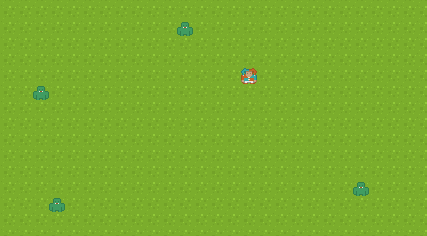
\includegraphics[width=0.5\textwidth]{data/ef/50772b-6721-4bd5-a274-efaba137299f/screenshot-20200406-225138.png}
\end{center}\end{center}
\end{frame}
\end{document}